%%%%%%%%%%%%%%%%%%%%%%%%%%%%%%%%%%%%%%%%%
% Jacobs Landscape Poster
% LaTeX Template
% Version 1.1 (14/06/14)
%
% Created by:
% Computational Physics and Biophysics Group, Jacobs University
% https://teamwork.jacobs-university.de:8443/confluence/display/CoPandBiG/LaTeX+Poster
% 
% Further modified by:
% Nathaniel Johnston (nathaniel@njohnston.ca)
%
% This template has been downloaded from:
% http://www.LaTeXTemplates.com
%
% License:
% CC BY-NC-SA 3.0 (http://creativecommons.org/licenses/by-nc-sa/3.0/)
%
%%%%%%%%%%%%%%%%%%%%%%%%%%%%%%%%%%%%%%%%%

%----------------------------------------------------------------------------------------
%	PACKAGES AND OTHER DOCUMENT CONFIGURATIONS
%----------------------------------------------------------------------------------------

\documentclass[final]{beamer}

\usepackage[scale=1.24]{beamerposter} % Use the beamerposter package for laying out the poster

\usepackage{multirow} % tables
\usepackage{booktabs}
\usepackage{array}

\usepackage[dvipsnames]{xcolor} % Use the xcolor package to define colors

\usetheme{confposter} % Use the confposter theme supplied with this template

\setbeamercolor{block title}{fg=MidnightBlue,bg=white} % Colors of the block titles
\setbeamercolor{block body}{fg=black,bg=white} % Colors of the body of blocks
\setbeamercolor{block alerted title}{fg=white,bg=dblue!70} % Colors of the highlighted block titles
\setbeamercolor{block alerted body}{fg=black,bg=dblue!10} % Colors of the body of highlighted blocks
% Many more colors are available for use in beamerthemeconfposter.sty

%-----------------------------------------------------------
% Define the column widths and overall poster size
% To set effective sepwid, onecolwid and twocolwid values, first choose how many columns you want and how much separation you want between columns
% In this template, the separation width chosen is 0.024 of the paper width and a 4-column layout
% onecolwid should therefore be (1-(# of columns+1)*sepwid)/# of columns e.g. (1-(4+1)*0.024)/4 = 0.22
% Set twocolwid to be (2*onecolwid)+sepwid = 0.464
% Set threecolwid to be (3*onecolwid)+2*sepwid = 0.708

\newlength{\sepwid}
\newlength{\onecolwid}
\newlength{\twocolwid}
\newlength{\threecolwid}
\setlength{\paperwidth}{48in} % A0 width: 46.8in
\setlength{\paperheight}{36in} % A0 height: 33.1in
\setlength{\sepwid}{0.024\paperwidth} % Separation width (white space) between columns
\setlength{\onecolwid}{0.22\paperwidth} % Width of one column
\setlength{\twocolwid}{0.464\paperwidth} % Width of two columns
\setlength{\threecolwid}{0.708\paperwidth} % Width of three columns
\setlength{\topmargin}{-0.5in} % Reduce the top margin size
%-----------------------------------------------------------

\usepackage{graphicx}  % Required for including images

\usepackage{booktabs} % Top and bottom rules for tables

%----------------------------------------------------------------------------------------
%	TITLE SECTION 
%----------------------------------------------------------------------------------------

\title{Can Multi-agent Collaboration Break the Curse of Complexity?} % Poster title

\author{{\normalsize Jack Speat \texttt{j.speat@sussex.ac.uk}} \\ {\footnotesize Supervised by Jeff Mitchell and Julie Weeds}} % Author(s)

\institute{\normalsize Department of Engineering and Informatics, University of Sussex} % Institution(s)

%----------------------------------------------------------------------------------------

\begin{document}

\addtobeamertemplate{block end}{}{\vspace*{2ex}} % White space under blocks
\addtobeamertemplate{block alerted end}{}{\vspace*{2ex}} % White space under highlighted (alert) blocks

\setlength{\belowcaptionskip}{2ex} % White space under figures
\setlength\belowdisplayshortskip{2ex} % White space under equations

\begin{frame}[t] % The whole poster is enclosed in one beamer frame

\begin{columns}[t] % The whole poster consists of three major columns, the second of which is split into two columns twice - the [t] option aligns each column's content to the top

\begin{column}{\sepwid}\end{column} % Empty spacer column

\begin{column}{\onecolwid} % The first column



%----------------------------------------------------------------------------------------
%	INTRODUCTION
%----------------------------------------------------------------------------------------

\begin{block}{Background}

    LLMs have shown limited performance across reasoning tasks when evaluated as individuals. Prior work by Yuchen et al. \cite{linZebraLogicScalingLimits2025} highlights a 'curse of complexity' scaling law in the context of reasoning.

%------------------------------------------------

    \begin{figure}
        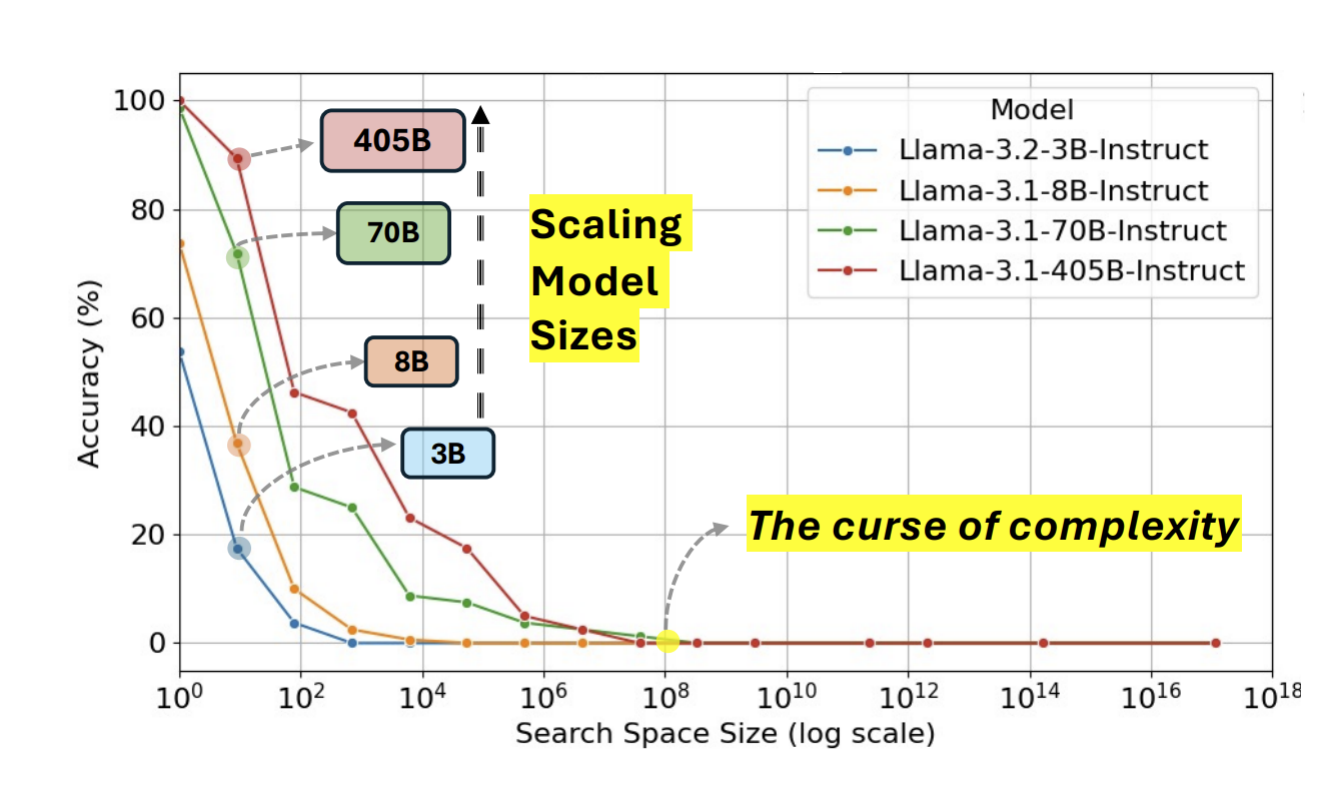
\includegraphics[width=0.8\linewidth]{figures/Curse of complexity.png}
        \caption{Scaling model size yields limited improvements on tasks higher in complexity \cite{linZebraLogicScalingLimits2025}}
    \end{figure}
    
%----------------------------------------------------------------------------------------

    Observation of human performance on logical reasoning tasks as individuals is similarly limited. \cite{moshmanCollaborativeReasoningEvidence1998} found that groups outperform the individuals that compose them on the Wason selection task. This phenomenon is sometimes referred to as the 'assembly bonus effect', wherein a group achieves better outcomes than its most competent individual.  

    \begin{figure}
        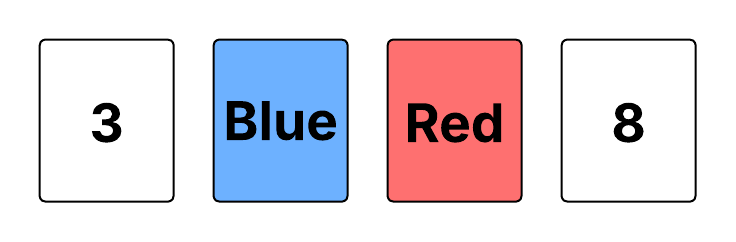
\includegraphics[width=0.8\linewidth]{figures/Wason.png}
        \caption{The Wason selection task}
    \end{figure}

    While the cognitive benefits of collaboration have been well-documented in human groups, it remains unclear whether similar effects can be observed in multi-agent systems composed of LLMs. 

\end{block}



%----------------------------------------------------------------------------------------
%	OBJECTIVES
%----------------------------------------------------------------------------------------

\begin{alertblock}{Research Questions}

    \begin{itemize}
    \item Do collaborative LLM agents outperform individual models as task complexity increases?
    \item Can groups of LLM agents collectively outperform their strongest individual member on reasoning tasks?
    \end{itemize}
    
    \end{alertblock}

\end{column} % End of the first column

\begin{column}{\sepwid}\end{column} % Empty spacer column

\begin{column}{\twocolwid} % Begin a column which is two columns wide (column 2)

% \begin{columns}[t,totalwidth=\twocolwid] % Split up the two columns wide column

% \begin{column}{\onecolwid}\vspace{-.6in} % The first column within column 2 (column 2.1)

%----------------------------------------------------------------------------------------
%	MATERIALS
%----------------------------------------------------------------------------------------

\begin{block}{Methods}

    \begin{figure}
        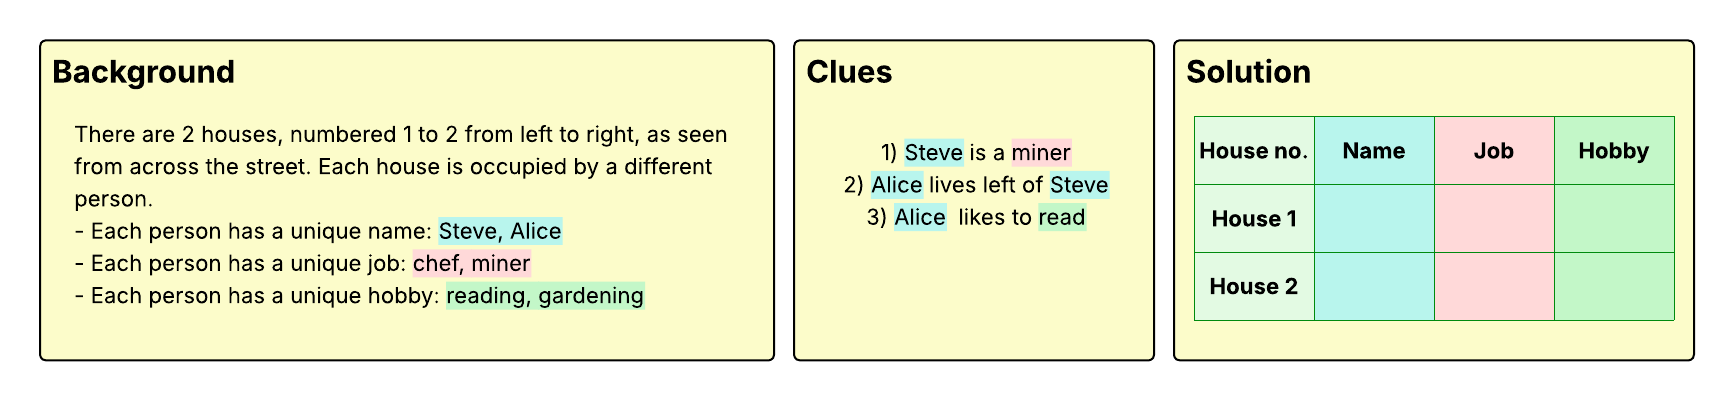
\includegraphics[width=0.8\linewidth]{figures/Example.png}
        \caption{Example ZebraLogic puzzle}
        \label{fig:example}
    \end{figure}

    ZebraLogic benchmark consists of logic grid puzzles derived from constraint satisfaction problems (CSPs). Fig. \autoref{fig:example} demonstrates a simple 2x3 problem. The task for the model is to determine the correct assignment of attributes to each house based on the clues given.  While this example is easily solvable using linear deduction, as complexity grows, non-monotonic reasoning strategies are required to successfully solve the puzzles. 
    
    \begin{figure}
        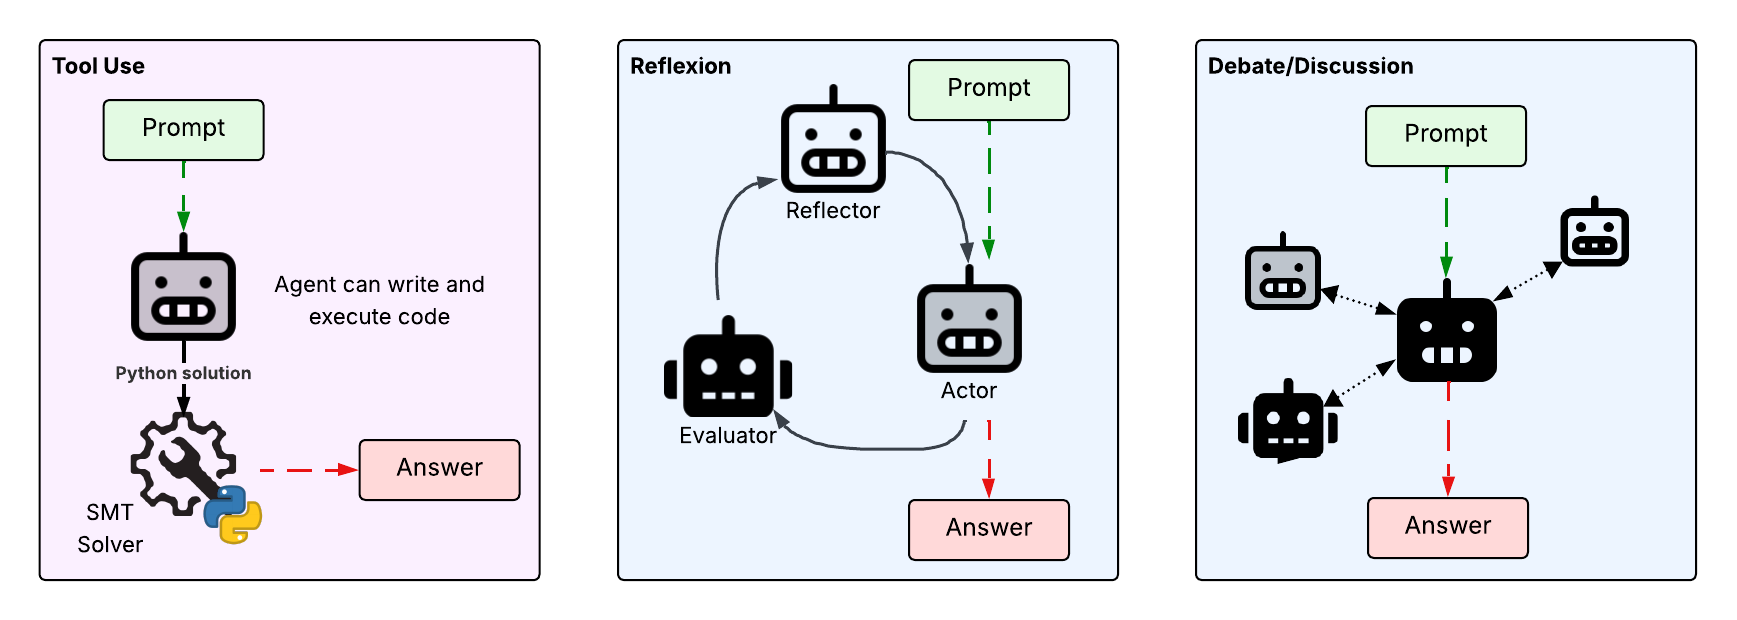
\includegraphics[width=0.8\linewidth]{figures/Solutions.png}
        \caption{From left to right: a single agent approach with tool use, a multi-agent reflection approach, and a collaborative approach.}
    \end{figure}
    
    Complexity can be measured using the size of the search space, where an \( N \times M \) grid has a solution space of size \( (N!)^M \), with \( N \) representing the number of houses and \( M \) the number of attributes. The puzzles can be categorised into groups based on the magnitude of the search space \( |S| \).

    Z3 conflicts can also be used as a complementary measure of complexity. This is the average number of situations in which the popular satisfiability modulo theories (SMT) solver has to backtrack due to contradictions in its current assignment. Puzzles with higher conflicts require extensive backtracking, indicating higher logical complexity. 



\end{block}
\vspace{-1em}
\begin{columns}[t,totalwidth=\twocolwid] % Split up the two columns wide column again

\begin{column}{\onecolwid} % The first column within column 2 (column 2.1)

%----------------------------------------------------------------------------------------
%	MATHEMATICAL SECTION
%----------------------------------------------------------------------------------------

\begin{block}{Metrics}

    Puzzle accuracy and cell-wise accuracy are measured to evaluate the completeness of the puzzle. 
    The length of the reasoning section of the answer will also be observed to see if reasoning length and puzzle complexity are correlated. 

\end{block}

%----------------------------------------------------------------------------------------

\end{column} % End of column 2.1

\begin{column}{\onecolwid} % The second column within column 2 (column 2.2)

%----------------------------------------------------------------------------------------
%	RESULTS
%----------------------------------------------------------------------------------------

\begin{block}{Experiment}

    To investigate the research questions, various architectures of multi-agent (MA) systems, and single LLMs will be tested using the ZebraLogic benchmark described above. The MA systems should only be comprised of the LLMs used as controls for a fair comparison. 

\end{block}

%----------------------------------------------------------------------------------------

\end{column} % End of column 2.2

\end{columns} % End of the split of column 2

\end{column} % End of the second column

\begin{column}{\sepwid}\end{column} % Empty spacer column

\begin{column}{\onecolwid} % The third column

%----------------------------------------------------------------------------------------
%	CONCLUSION
%----------------------------------------------------------------------------------------

\begin{block}{Preliminary Results}
    {\footnotesize
    \begin{table}[h!]
        \centering
        \begin{tabular}{|l|c|c|c|}
        \hline
        \textbf{Model} & \textbf{Format} & \textbf{Puzzle Acc.} & \textbf{Cell Acc.} \\
        \hline
        \multirow{2}{*}{7B Math} & JSON & 15.63 & 25.63 \\
                                & XML & 2.19 & 1.91 \\
        \hline
        \multirow{2}{*}{7B Instruct} & JSON & 35.62 & 64.92 \\
                                & XML & 32.19 & 63.81 \\
        \hline
        \multirow{2}{*}{14B Code} & JSON & 43.44 & 70.32 \\
                                & XML & 34.69 & 69.13 \\
        \hline
        \multirow{2}{*}{14B Instruct} & JSON & 57.81 & 79.25 \\
                                & XML & 58.44 & 79.33 \\
        \hline

        \end{tabular}
        \caption{Subset of results. All models are in the Qwen2.5 family.}
    \end{table}
    }
    An initial experiment evaluated the performance of LLMs on the ZebraLogic task when prompted to output solutions in either JSON or XML format. 


\end{block}

%----------------------------------------------------------------------------------------
%	ADDITIONAL INFORMATION
%----------------------------------------------------------------------------------------

\begin{block}{Next Steps}

    Future work will apply the current experimental framework to a broader range of logical reasoning tasks to assess whether the observed patterns generalise across different problem types and domains. This will help evaluate the robustness of collaborative LLM agent performance and the potential applicability of the assembly bonus effect beyond the initial task setting.

\end{block}

%----------------------------------------------------------------------------------------
%	REFERENCES
%----------------------------------------------------------------------------------------

\begin{block}{References}

\nocite{*} % Insert publications even if they are not cited in the poster
\small{\bibliographystyle{unsrt}
\bibliography{sample}\vspace{0.75in}}

\end{block}

%----------------------------------------------------------------------------------------
%	ACKNOWLEDGEMENTS
%----------------------------------------------------------------------------------------

\setbeamercolor{block title}{fg=red,bg=white} % Change the block title color

\begin{block}{Acknowledgements}

\small{\rmfamily{This research is supported by SussexAI through the SussexAI Studentship}} \\

\end{block}

%----------------------------------------------------------------------------------------
%	CONTACT INFORMATION
%----------------------------------------------------------------------------------------

\setbeamercolor{block alerted title}{fg=black,bg=norange} % Change the alert block title colors
\setbeamercolor{block alerted body}{fg=black,bg=white} % Change the alert block body colors




\begin{tabular}{ccc}

\includegraphics[width=0.8\linewidth]{figures/sussex_ai_cover.jpeg} 
\end{tabular}

%----------------------------------------------------------------------------------------

\end{column} % End of the third column

\end{columns} % End of all the columns in the poster

\end{frame} % End of the enclosing frame

\end{document}
